%% ****** Start of file template.aps ****** %
%%
%%
%%   This file is part of the APS files in the REVTeX 4 distribution.
%%   Version 4.0 of REVTeX, August 2001
%%
%%
%%   Copyright (c) 2001 The American Physical Society.
%%
%%   See the REVTeX 4 README file for restrictions and more information.
%%
%
% This is a template for producing manuscripts for use with REVTEX 4.0
% Copy this file to another name and then work on that file.
% That way, you always have this original template file to use.
%
% Group addresses by affiliation; use superscriptaddress for long
% author lists, or if there are many overlapping affiliations.
% For Phys. Rev. appearance, change preprint to twocolumn.
% Choose pra, prb, prc, prd, pre, prl, prstab, or rmp for journal
%  Add 'draft' option to mark overfull boxes with black boxes
%  Add 'showpacs' option to make PACS codes appear
\documentclass[aps,prl,twocolumn,showpacs,superscriptaddress,groupedaddress]{revtex4}  % for review and submission
%\documentclass[aps,preprint,showpacs,superscriptaddress,groupedaddress]{revtex4}  % for double-spaced preprint
\usepackage{graphicx}  % needed for figures
\usepackage{dcolumn}   % needed for some tables
\usepackage{bm}        % for math
\usepackage{amssymb}   % for math
%\usepackage{psfrag}
%\usepackage{epsf}
% avoids incorrect hyphenation, added Nov/08 by SSR
\hyphenation{ALPGEN}
\hyphenation{EVTGEN}
\hyphenation{PYTHIA}


\begin{document}

% The following information is for internal review, please remove them for submission
\widetext
\leftline{Version xx as of \today}
\leftline{Primary authors: Joe E. Physics}
\leftline{To be submitted to PRL}
\leftline{Comment to {\tt d0-run2eb-nnn@fnal.gov} by xxx, yyy}
\centerline{\em D\O\ INTERNAL DOCUMENT -- NOT FOR PUBLIC DISTRIBUTION}

% the following line is for submission, including submission to the arXiv!!
%\hspace{5.2in} \mbox{Fermilab-Pub-04/xxx-E}

\title{Two dimensional elastic turbulence}
\date{\today}


\begin{abstract}
In this paper, by smoothed dissipative particle dynamics(SDPD), we investigate the properties of polymer solution caused by intorducing polymer in solvent 
in two-dimensional Kolmogorov flow.\\
In polymer solution, we observe a disordered, turbulentlike mixing flow in
Kolmogorov flow at high Weissenbergnumber($Wi\approx29$) and small Reynolds numbers($Re\approx1$), at which the solvent flow is laminar.
We capture the vortex and energy spectrum with scaling law in this case,which proves that the instability of flow caused by polymers is formed in our simulation.
\end{abstract}

\pacs{}
\maketitle

%\section{\label{sec:level1}First-level heading}
% sections are not used for PRL papers
It is well known that the addition fo small amounts of long chain polymers can have a strong impact on flowing fluid's properties.
One of the most remarkable effects of highly viscous polymer solutions which has been
observed in experiments is the development of an elastic turbulence regime in the limit of small Reynolds number and strong 
elasticity \cite{groisman00}. The flow in this regime displays a rich dynamics, of the type usually encountered
in high Reynolds number turbulent flow in Newtonian fluids. Typical features of turbulent flows (e.g.,broad
range of active scales, growth of flow resistance) are observed in the experiments by Steinberg and collaborators \cite{groisman00},
even at low velocity and high viscosity, i.e. in the limit of vanishing Reynolds number. As a consequence of 
turbulent-like motion, elastic turbulence has been proposed as an efficient technique for mixing in very
low Reynolds flows, such as in microchannel flows \cite{groisman01}. Despite its great technological interest, elastic turbulence
is still only partially understood from a theoretical point of view. Presently available theoretical predictions are
based on simplified versions of viscoelastic models and on the analogy with magnetohydrodynamics (MHD) equations \cite{balk01}\cite{fouxon03}. 
It has recently been successfully captured by direct numerical simulation based on Oldroyd-B model in a two-dimensional viscoelastic flow \cite{berti08}.
Note that in DNS simulation they use linear viscoelastic model(Oldroyd-B). In this paper we use FENE-P model,which is more accurate and accounts for the nonlinear character of polymer
elasticity,culminating in a finite molecular extensibility\cite{bird87}.\\
SDPD method is a particle model that is both thermodynamically consistent version of smoothed particle hydrodynamics(SPH) and a version of dissipative particle dynamics(DPD)
\cite{pep03}.The equations of SDPD in mesoscopic hydrodynamics are \cite{hu06}
%The pressure effect on the velocity
%\begin{equation}\label{equ:momeevo}
% \frac{d\mathbf{v}_{i}^{(p)}}{dt}=-\frac{1}{m_i}\sum_j(\frac{p_i}{d_{i}^{2}}+\frac{p_j}{d_{j}^{2}})\frac{\partial W}{\partial r_{ij}}\mathbf{e}_{ij},
%\end{equation}
%where $\frac{d\mathbf{v}_{i}^{(p)}}{dt}$ is the particle acceleration caused by pressure
%effects
%The viscosicty effect on the velocity is 
%\begin{equation}\label{equ:acceleration}
 %\frac{d\mathbf{v}{_i}{^{(\upsilon)}}}{dt}=-\frac{\eta}{m_i}\sum_j\left(\frac{p^i}{d_{i}^{2}}+\frac{p^j}{d_{j}^{2}}\right)\frac{\partial W}{\partial r_ij}(\mathbf{e}_{ij}\cdot\mathbf{v}_{ij}\mathbf{e}_{ij}+\mathbf{v}_{ij}),
%\end{equation}
%the thermal fluctuation part is :
%\begin{equation}\label{equ:thermalb}
 %d\tilde{m}_i=0,
%d\tilde{\mathbf{P}}_i=\sum_j B_{ij}d\bar{\mathcal{W}}_{ij}\cdot\mathbf{e}_{ij}
%\end{equation}
%\begin{equation}\label{equ:thermalfur}
 % \dot{m}_i\vert_{irr}=0,
%\dot{\mathbf{P}}_i\vert_{irr}=-\sum_j\frac{B_{ij}}{4k_BT}
%(\mathbf{e}_{ij}\cdot\mathbf{v}_{ij}\mathbf{e}_{ij}+\mathbf{v}_{ij}),
%\end{equation}
%in which $k_B$ is the Boltzmann constant and $T$ is the system temperature and 
%$B_{ij}=[-4k_BT\eta(\frac{1}{d_{i}^{2}}+\frac{1}{d_{j}^{2}})r_{ij}\frac{\partial W}{\partial r_{ij}}]^{1/2}.$
%so the equation can be written into:
\begin{eqnarray}\label{equ:momesum}
 \frac{d\mathbf{r}_i}{dt}=\mathbf{v}_i,\\
\frac{d\mathbf{v}_i}{dt}=\frac{d\mathbf{v}_{i}^{(p)}}{dt}+\frac{d\mathbf{v}_{i}^{(\upsilon)}}{dt}+\frac{1}{m_i}d\tilde{\mathbf{P}}_i,
\end{eqnarray}
where $\mathbf{r}_i,\mathbf{v}_i,m_i$ are position, velocity and mass of a particle $i$,respectively.
$\frac{d\mathbf{v}_{i}^{(p)}}{dt},\frac{d\mathbf{v}_{i}^{(\upsilon)}}{dt},\frac{1}{m_i}d\tilde{\mathbf{P}}_i $ are partilce acceleration caused by pressure,
viscous force and thermal fluctuation,respectively.
The solvent liquid is represented by SDPD partilces which represents physical elements of fluid containing potentially thousands of solvent(i.e.,water)
 molecules and interacting hydrodynamically.Concerning the polymer model,we consider it as a linear chain of polymer beads,each bead 
being represented as a mixture of real polymer monomers together with solvent molecules.The numberical realization of this physical model is obtained by selecting a number of
SDPD fluid particles and letting them interact,as well as hydrodynamically, also by addtional finitely extendable nonlinear elastic springs(FENE) 
\begin{equation}\label{equ:fene}
 \mathbf{F}^{FENE}(\mathbf{r}_{ij})=\frac{K\mathbf{r}_{ij}}{1-(r/R_0)^2}
\end{equation}
where $K$ is the spring constant,$r=\sqrt{\mathbf{r}_{ij}\mathbf{r}_{ij}}$ is the bead-bead
distance, and $R_0$ represents the maximum extensibility of polymer molecules.\\
The periodic Kolmogorov flow is useful to study the elastic turbulence regime for visoelastic flows,withing force $\mathbf{F}=(F_0cos(k_yy),0)$,
where $k_y= 2\pi/L$ is the wave vector and $L$ is the length of the simulation box in the $y$-direction. A theoretical solution can be obtained for the 
velocity field which has the same functional form as the perturbation $\mathbf{v}=(v_0sin(k_yy),0)$
with $ v_0=F_0/\upsilon k_{y}^{2}$ and $\upsilon$ is the kinematic viscosity,which includes the solvent viscosicty and yero-shear contribution of polymers to the total solution viscosity. Nevertheless, for increasing values of the applied force $F_0$,
the Kolmogorov flow is known to be unstable and a secondary steady flow appears which consists of a periodic configuration of stationary vortices \cite{posch97}.
Indeed, a remarkable feature of the Kolmgorov flow is that even in the turbulent regime the mean velocity are accurately described by sinusoidal frofiles\cite{boffetta05}.
Here for this particular flow, the Reynolds number $Re=\frac{UL}{\upsilon}$ and the Weissenberg number $Wi=\frac{UL}{\tau}$, are defined in term of the amplitude U of the mean velocity,which is 
measured from the velocity profiles,$\tau$ is relaxation time of polymer.

First we check the physical phenomenon in solvent at vanishing Renold number.At Re=1.0
we get the enegy spectrum,Fig.\ref{fig:spesols}\\As we know in small renold number,and the same time the viscosity of the flow is small,the energy density will be the same 
along the scale,so the energy in two dimensional will be propotional to wavenumber.
\begin{figure}
 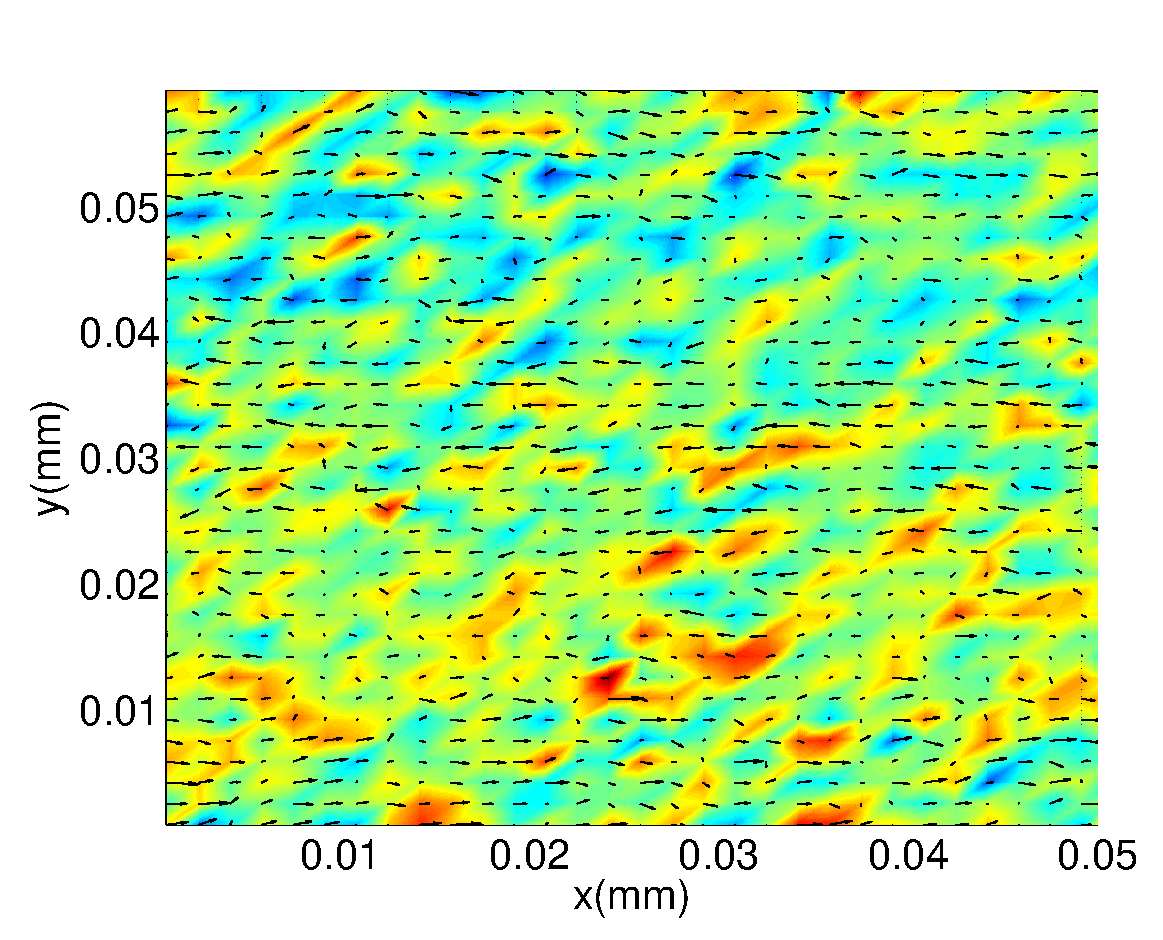
\includegraphics[scale=0.5]{vorsols}
\label{fig:spesols}
\caption{Vorticity field in solvent at Re=1}
\end{figure} \\
\begin{figure}
 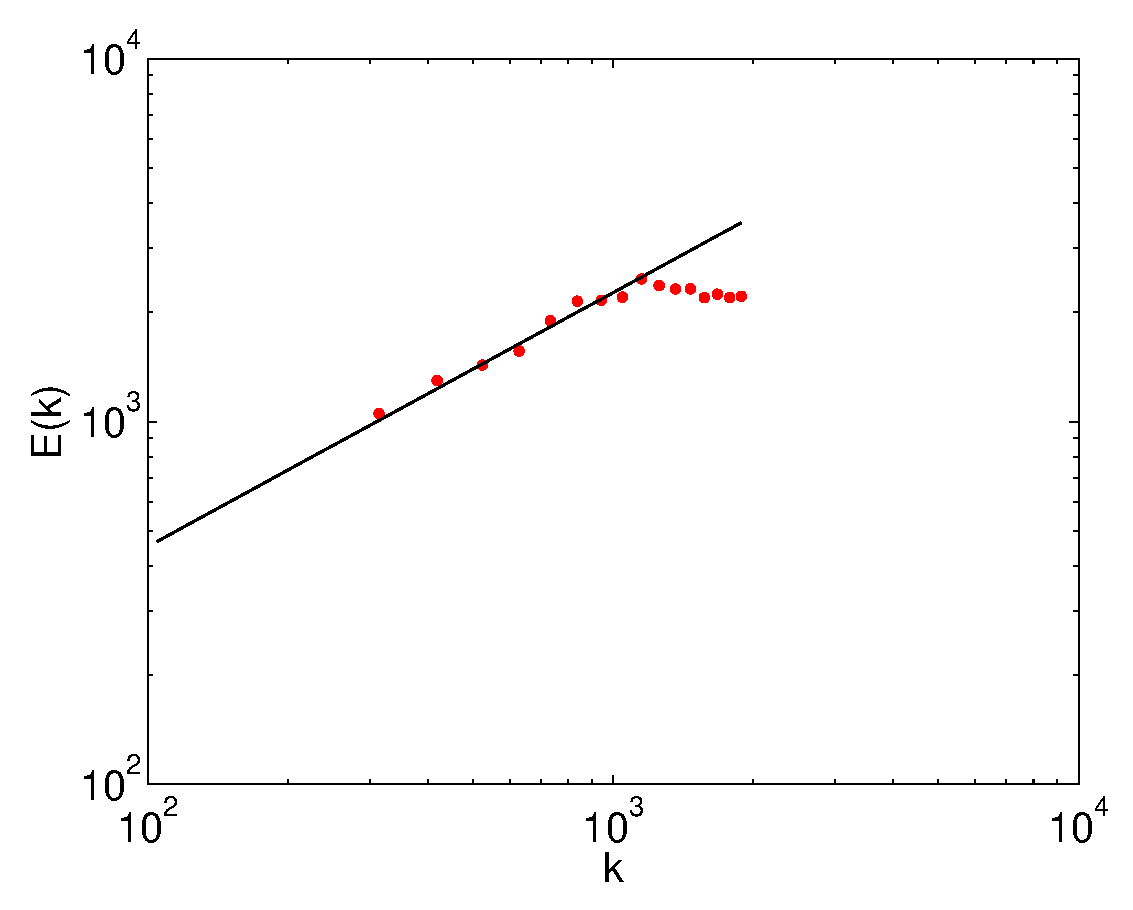
\includegraphics[scale=0.5]{spesols}
\label{fig:spesols}
\caption{Enegy spectrum in solvent at Re=1}
\end{figure} \\

Polymer solution--At Re=1 Wi=29 we get the vorticity field and spectrum,Fig.\ref{fig:spepols}
From the picture we can see the vortex structure is not sontinous,this may be resulted from the small domain and the length of polymer is short.
The energy spectrum is k-1,which is not the same as in the DNS simulation.The reason is the model of the polymer is different,in DNS is Oldroyd-B,in ouy case is more accurate model
FENE-P model.Then another reason is the viscosicty in our case is 0.5,and the resolution is small(32*32).
model
\begin{figure}
 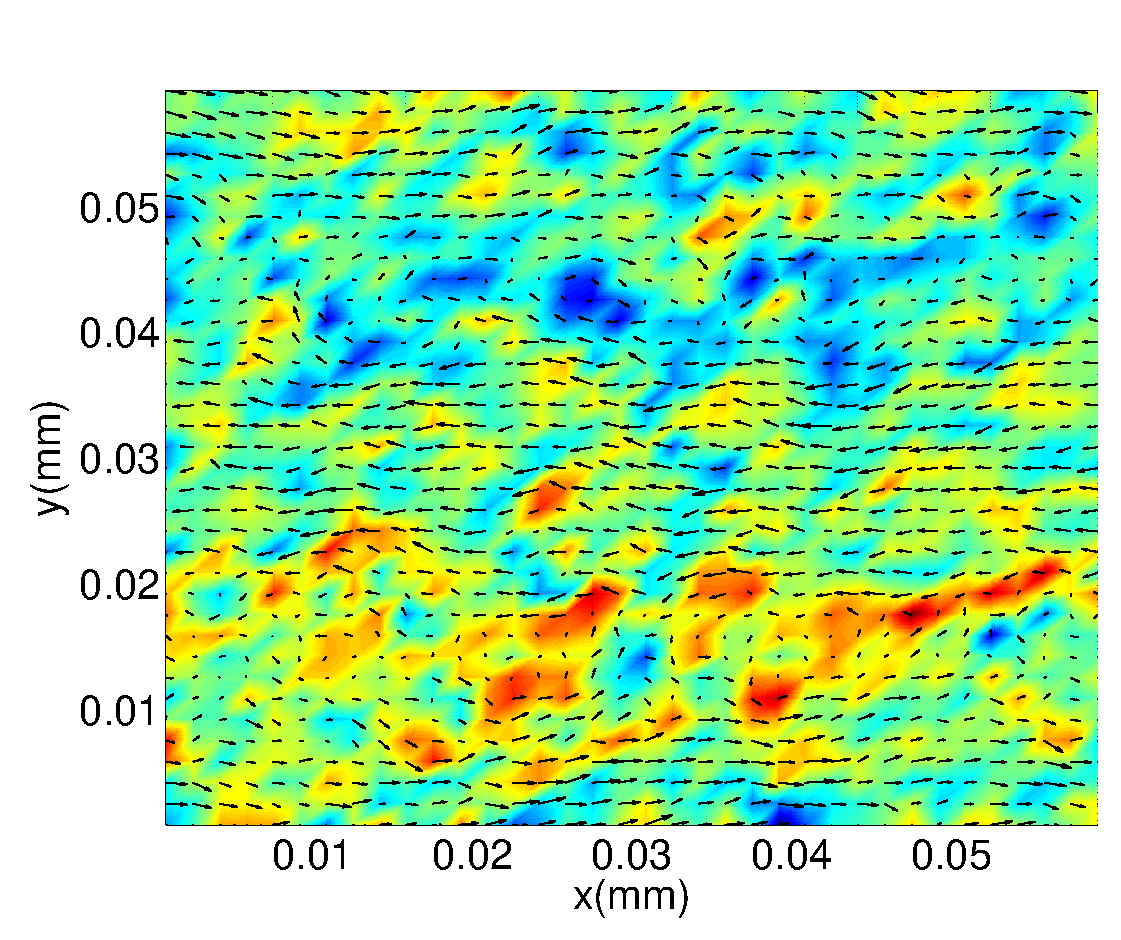
\includegraphics[scale=0.5]{vorpols}
\label{fig:vorpols}
\caption{Energy spectrum in polymer solution at Re=1,Wi=30}
\end{figure}\\
\begin{figure}
 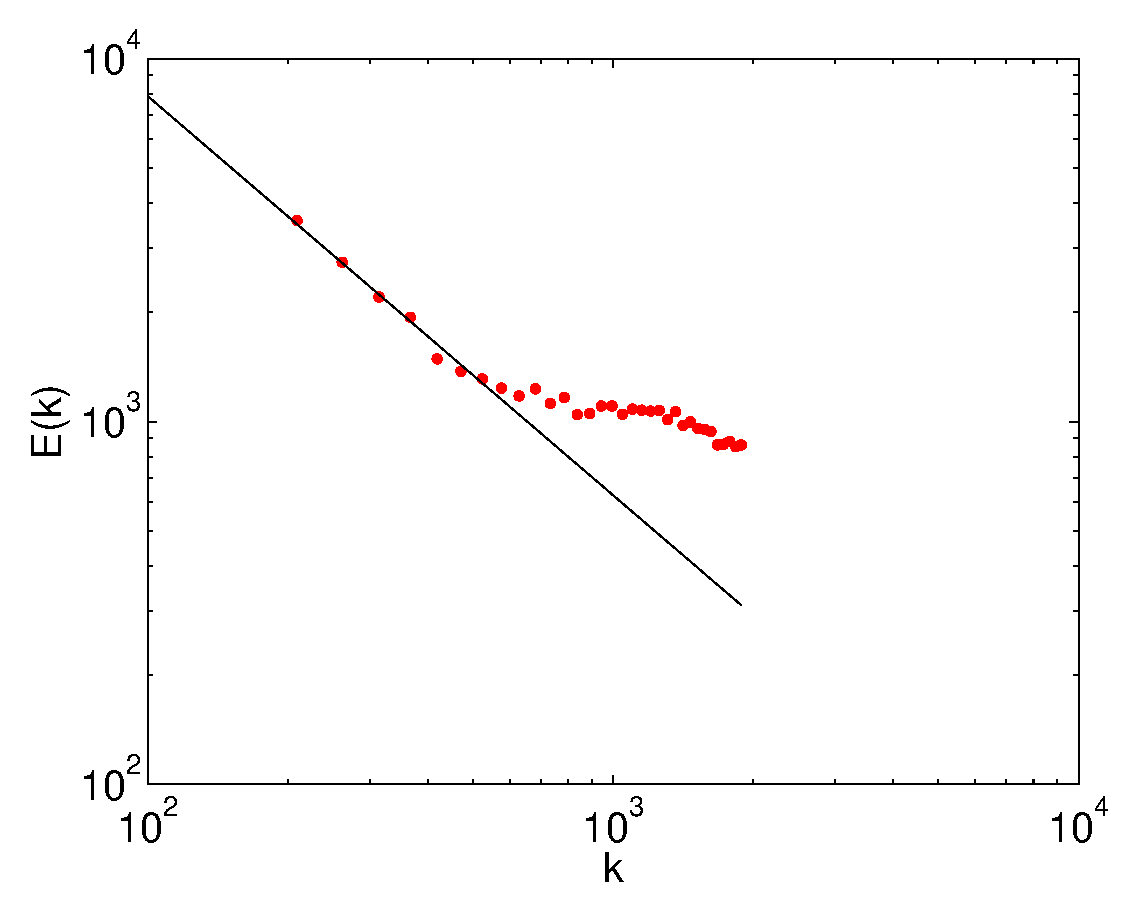
\includegraphics[scale=0.5]{spepols}
\label{fig:spepols}
\caption{Energy spectrum in polymer solution at Re=1,Wi=30}
\end{figure}\\
The relaxation time of polymer 
 $\tau$ is relaxation time of polymer,which is 
calculated from the fitting of autocorrelation functio of end to end distance vector of polymer in a thermal stochastic simulaiton.
The investigation based on longer polymer molecules and high viscosicty will be presented in further work.
\bibliography{elt}
\bibliographystyle{unsrt}
\end{document}
%
% ****** End of file template.aps ******
